\documentclass[11pt,letterpaper]{article}
\usepackage[english]{babel}
\usepackage[utf8]{inputenc}
\usepackage{fancyhdr}
\usepackage[margin=1in]{geometry}
\usepackage{enumitem}
\usepackage{amsmath}
\usepackage{setspace} 
\usepackage{graphicx}
\onehalfspacing
 
 
\pagestyle{fancy}
\fancyhf{}
\lhead{AMATH 383 Homework 2}
\rhead{Nan Tang (1662478)}
\rfoot{Page \thepage}

\title{AMATH 383 Homework 2}
\author{Nan Tang \\ University of Washington}
\date{\today}

\begin{document}
\maketitle

\section*{Exercise 9.4}
\subsection*{a}
Solve this set of differential equation through dividing $\frac{dy}{dt}$ by $\frac{dx}{dt}$. 
\begin{align*}
\frac{dy}{dt} / \frac{dx}{dt} &= \frac{-bx}{-axy} \\
\frac{dy}{dx} &= \frac{b}{ay} \\
(ay )dy &=( b) dx 
\end{align*}
\noindent Integrate both sides of this equation, and let $y_0, x_0$ denote the initial value for $y(t), x(t)$.
\begin{align*}
\int_{y_0}^{y(t)}( ay )dy &= \int_{x_0}^{x(t)}( b )dx \\
\frac{a}{2}( y(t)^2 - y_0^2) &= b(x(t) - x_0) \\
b x(t) &= \frac{a}{2} y(t)^2  - \frac{a}{2} y_0^2) + bx_0\\
x(t) &= \frac{a}{2b} y(t)^2 + (x_0 - \frac{a}{2b} y_0^2)
\end{align*}
\noindent The last equation shows the relation between $x(t)$ and $y(t)$ is a parabola equation. The intercept of this parabola on x and y axis is determined by the constant $(x_0 - \frac{a}{2b} y_0^2)$. \\

\noindent Since the derivatives of both $x(t)$ and $y(t)$ is negative, as $t$ grows, $x(t)$ and $y(t)$ will go down to zero. In this model, the war ends until any of the side is eliminated. A stale means $y(t)$ and $x(t)$ arrive at zero simultaneous, i.e. no one left for both sides. \\

\noindent Let $K = (x_0 - \frac{a}{2b} y_0^2)$, and plot the $x(t)y(t)$ relationship. 

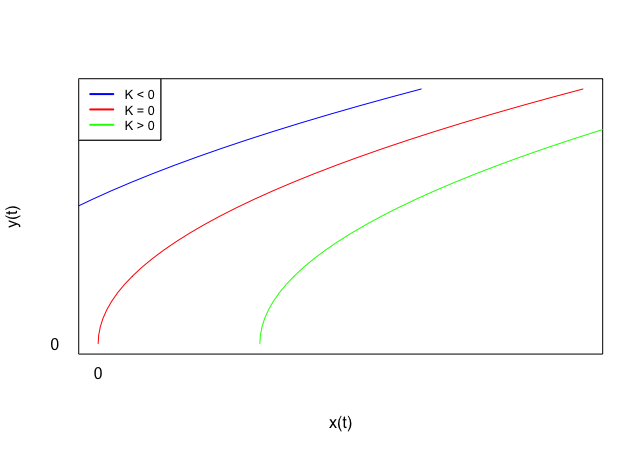
\includegraphics[scale=0.6]{1-a-1.png}

\noindent Base on the graph, when $K < 0$, the solution ends on y-axis, indicating y wins; when $K > 0$, the solution line hits the x-axis, implying x wins. A stale will happen only if $x_0 - \frac{a}{2b} y_0^2 = 0$, since the solution goes into $y(t) = x(t) = 0$. \\

\noindent Note that $a = c_1 \frac{A_g}{A_x}$ where $A_g = 2, A_x = 1000 \cdot x_0$; $b = c_2 p_x$ where $p_x = 0.1, c_1 = c_2$.
\begin{equation*}
x_0 - \frac{a}{2b} y_0^2 = x_0 - \frac{c_1 A_g}{ 2 A_x \cdot c_2 p_x} y_0^2 = x_0 - \frac{1}{100 x_0} y_0^2
\end{equation*}
\noindent $x_0$ and $y_0$ denotes the initial force. When $y_0$ is ten times $x_0$, a stale will occur. \\

\subsection*{b}
\noindent From the previous question, we know that when $x_0 - \frac{a}{2b} y_0^2 < 0$, the solution will ends up on y-axis as $t$ is big enough. In this case, $y$ wins since $x$ loses all its force but $y$ still has remaining power. \\

\noindent Plug in the value of $a, b, c_1, c_2$, we get 
\begin{align*}
x_0 - \frac{a}{2b} y_0^2  &< 0 \\
x_0 &< \frac{1}{100 x_0} y)^2 \\
x_0 &< \frac{1}{10} y_0
\end{align*}
\noindent When initial force of y is more than 10 times of $x_0$, y will win the battle. \\

\noindent The true initial values are $y^*_0 \leq 6 x^*_0$. Since y wins only if $y_0 \geq 10 x_0$, US cannot prevail in the war. 

\section*{Exercise 9.5}
\subsection*{a}
\noindent Given that $\frac{dN}{dt} = rN(1 - \frac{N}{K} ) - \beta N$ and $N(t) = x(t) + y(t)$, we can replace $N(t)$ by $x(t), y(t)$.
\begin{align*}
\frac{d N}{dt} &= r(x + y) (1 - \frac{x + y}{K} )- \beta (x + y) \\
&= (x + y) (r - \frac{r (x + y)}{K} )- \beta (x + y)
\end{align*}
\noindent Note that $\frac{d N}{dt} = \frac{dy}{dt} + \frac{dx}{dt}$, therefore the only possible equation for $F(x, y)$ that satisfies $\frac{dx}{dt} = x F(x,y) + \beta x$ and $\frac{dy}{dt} = y F(x,y) + \beta y$ is $F(x, y) = r(1 - \frac{x + y}{K})$ \\

\subsection*{b}
\noindent The new model looks like 
\begin{align*}
\frac{dx}{dt} &= x[r (1 - \frac{x + y}{K}) - \beta] \\
\frac{dy}{dt} &= y[r(1 - \frac{x+y}{K}) - \beta (1 - \epsilon)]
\end{align*}
\noindent To find the equilibrium points, we want both $\frac{dx}{dt}$ and $\frac{dy}{dt}$ to be zero. \\

\noindent There are four possible equilibrium solutions: $x=0, y=0$; $x=0, r(1 - \frac{x+y}{K}) - \beta (1 - \epsilon)=0$; $r (1 - \frac{x + y}{K}) - \beta=0, y=0$ and $r (1 - \frac{x + y}{K}) - \beta=0, r(1 - \frac{x+y}{K}) - \beta (1 - \epsilon)=0$\\

\noindent \textbf{Equilibria 1} $(x^*, y^*) = (0, 0)$ \\

\noindent when $x=0, r(1 - \frac{x+y}{K}) - \beta (1 - \epsilon)=0$
\begin{align*}
r(1 - \frac{y}{K}) - \beta (1 - \epsilon) &= 0 \\
y &= K - \frac{K}{r} \beta (1 - \epsilon)
\end{align*}

\noindent \textbf{Equilibria 2}  $(x^*, y^*) = (0, K - \frac{K}{r} \beta (1 - \epsilon))$ \\

\noindent when  $r (1 - \frac{x + y}{K}) - \beta=0, y=0$
\begin{align*}
r (1 - \frac{x}{K}) - \beta &=0 \\
x &= K - \frac{K}{r} \beta
\end{align*}
\noindent \textbf{Equilibria 3}  $(x^*, y^*) = (K - \frac{K}{r} \beta, 0)$ \\

\noindent when $r (1 - \frac{x + y}{K}) - \beta=0, r(1 - \frac{x+y}{K}) - \beta (1 - \epsilon)=0$, there is not solution for $x, y$ to satisfy this condition. \\

\noindent In summary, there are three equilibrium points for this model, they are $(0, 0), (0, K - \frac{K}{r} \beta (1 - \epsilon)), (K - \frac{K}{r} \beta, 0)$ \\

\subsection*{c}
\noindent First get the matrix $A$ for linear analysis.
\begin{itemize}
\item $a_{11} = \frac{\partial f}{\partial x} = r (1 - \frac{x+y}{K}) - \beta - \frac{r}{K} x$ 
\item $a_{12} = \frac{\partial f}{\partial y} = - \frac{r}{K}x$
\item $a_{21} = - \frac{r}{K} y$
\item $a_{22} = r (1 - \frac{x+y}{K}) - \beta (1 - \epsilon) - \frac{r}{K} y$
\end{itemize}

\noindent \textbf{Equilibria 1} $(x^*, y^*) = (0, 0)$ \\

\noindent $a_{11} = r - \beta$, $a_{12} = 0$ $a_{21} = 0$, $a_{22} = r - \beta (1 - \epsilon)$ 

\noindent $p = a_{11} + a_{22} = 2 r - \beta (2 - \epsilon)$

\noindent $q = a_{11}a_{a22} - a_{12} a_{21} = (r - \beta)(r - \beta(1 - \epsilon))$\\

\noindent Note that $\lambda_1 = \frac{p}{2} + \frac{\sqrt{p^2 - 4q}}{2}$, $r > \beta > \beta (1 - \epsilon)$, therefore $\lambda_1 > \frac{p}{2} > 0 $. Point $(0, 0)$ is unstable. \\

\noindent \textbf{Equilibria 2}  $(x^*, y^*) = (0, K - \frac{K}{r} \beta (1 - \epsilon))$ \\

\noindent $a_{11} = - \beta \epsilon$, $a_{12} = 0$, $a_{21} = \beta (1 - \epsilon) - r$, $a_{22} = \beta (1 - \epsilon) - r$

\noindent $p = a_{11} + a_{22} = \beta - r - 2 \beta \epsilon $

\noindent $q =  a_{11}a_{a22} - a_{12} a_{21} = r \beta \epsilon - \beta^2 \epsilon + \beta^2 \epsilon^2 $ \\


\noindent In this case, $p < 0$ and $\sqrt{p^2 - 4q} < - p $. Therefore, both $\lambda_1$ and $\lambda_2$ are less than zero. The equilibrium point $(0, K - \frac{K}{r} \beta (1 - \epsilon))$ is stable. \\

\noindent \textbf{Equilibria 3}  $(x^*, y^*) = (K - \frac{K}{r} \beta, 0)$ \\

\noindent $a_{11} = \beta - r$, $a_{12} = \beta - r$, $a_{21} = 0$, $a_{22} = \beta \epsilon$ 

\noindent $p = a_{11} + a_{22} = \beta -r + \beta \epsilon$

\noindent $q =  a_{11}a_{a22} - a_{12} a_{21} = (\beta - r) \beta \epsilon$ \\

\noindent $\lambda_1 = \frac{1}{2}(p + \sqrt{p^2 - 4q}) = \frac{1}{2} (\beta - r + \epsilon + \beta - r - \epsilon) = \beta - r < 0$

\noindent $\lambda_2 = \frac{1}{2}(p - \sqrt{p^2 - 4q}) = \frac{1}{2} (\beta - r + \epsilon - \beta + r + \epsilon) = \epsilon > 0$ \\

\noindent In this case, $\lambda_2 > 0$, thus the point $(K - \frac{K}{r} \beta, 0)$ is unstable. \\

\subsection*{d}
\noindent From previous question, we can perceive that the only stable equilibrium point for this dynamic system is $x^* = 0$ and $y^* =K - \frac{K}{r} \beta (1 - \epsilon) $. As time goes on, $x$, representing population of Neanderthals, will finally go to zero, and the population of human $y$ will converge to a stable point $K - \frac{K}{r} \beta (1 - \epsilon) $ which is determined by growth rate, mortality rate and carry capacity. Therefore, the extinction of Neanderthals is inevitable. \\

\subsection*{e}
\begin{align*}
\frac{d}{dt} ( \frac{x(t)}{y(t)} )&= \frac{1}{y} \frac{dx}{dt} - \frac{x}{y} \frac{1}{y} \frac{dy}{dt} \\
&= \frac{x}{y} (r(1 - \frac{x+y}{K}) - \beta) - \frac{x}{y} (r(1 - \frac{x + y}{K}) - \beta (1 - \epsilon)) \\
&= - \beta \epsilon ( \frac{x(t)}{y (t)} )
\end{align*}
\noindent Solution for this ODE is $\frac{x(t)}{y(t)} = (\frac{x(t_0)}{y(t_0)}) e ^{- \beta \epsilon t}$. Let $A_0$ denotes initial condition $\frac{x(t_0)}{y(t_0)}$, then the solution becomes $\frac{x(t)}{y(t)} = A_0 e^{-\epsilon \beta t}$. \\

\noindent Note that at $t = 10000$, $\frac{x(t)}{y(t)} = A_0 / e$ and $\beta = \frac{1}{30}$, we can get equation:
\begin{align*}
A_0 e^{- \epsilon \beta t} &= A_0 / e \\
e^{- \frac{10000}{30} \epsilon} &= e^{-1} \\
\epsilon &= \frac{30 }{10000} = 0.003
\end{align*}
\noindent The mortality difference between humans and Neanderthals is 0.003.








\end{document}